\documentclass[conference,a4paper]{IEEEtran}
\IEEEoverridecommandlockouts
\usepackage[T1]{fontenc}
\usepackage[utf8]{inputenc}
\usepackage[brazil]{babel}
\usepackage{amsmath,amssymb}
\usepackage{graphicx}
\usepackage{booktabs}
\usepackage{array}
\usepackage{cite}
\usepackage{url}
\usepackage[hidelinks]{hyperref}
\graphicspath{{../figuras/}}
\renewcommand\IEEEkeywordsname{Palavras-chave}
\hypersetup{pdftitle={Triagem de cardiopatia pediátrica sem vazamento de dados},
  pdfauthor={Murilo Uchôa, Felipe Orlow e João Henrique Simielli}}

% Gerado por src/artefatos.py a partir de resultados/ — não editar à mão.
\makeatletter
\providecommand{\defnum}[2]{\@namedef{num@#1}{#2}}
\providecommand{\dado}[1]{\@ifundefined{num@#1}{\PackageError{numeros}{Numero indefinido: #1}{}}{\@nameuse{num@#1}}}
\makeatother
\defnum{ano-fim}{2010}
\defnum{ano-ini}{2003}
\defnum{atributos-brutos}{21}
\defnum{atributos-modelo}{13}
\defnum{aucuni-altura}{0{,}638}
\defnum{aucuni-b2}{0{,}549}
\defnum{aucuni-convenio}{0{,}570}
\defnum{aucuni-fc}{0{,}636}
\defnum{aucuni-hda1}{0{,}561}
\defnum{aucuni-idade}{0{,}627}
\defnum{aucuni-imc}{0{,}600}
\defnum{aucuni-motivo1}{0{,}683}
\defnum{aucuni-motivo2}{0{,}721}
\defnum{aucuni-pamedida}{0{,}553}
\defnum{aucuni-peso}{0{,}646}
\defnum{aucuni-ppa}{0{,}546}
\defnum{aucuni-pulsos}{0{,}509}
\defnum{aucuni-sexo}{0{,}511}
\defnum{aucuni-sopro}{0{,}908}
\defnum{ausencia-altura}{30{,}1\%}
\defnum{ausencia-convenio}{27{,}5\%}
\defnum{ausencia-fc}{6{,}2\%}
\defnum{ausencia-hda1}{25{,}9\%}
\defnum{ausencia-idade}{6{,}7\%}
\defnum{ausencia-imc}{33{,}5\%}
\defnum{ausencia-motivo1}{1{,}2\%}
\defnum{ausencia-motivo2}{22{,}1\%}
\defnum{ausencia-pamedida}{0{,}0\%}
\defnum{ausencia-peso}{17{,}1\%}
\defnum{ausencia-ppa}{0{,}0\%}
\defnum{ausencia-pulsos}{0{,}3\%}
\defnum{ausencia-sexo}{4{,}5\%}
\defnum{convenio-antes}{367}
\defnum{convenio-depois}{228}
\defnum{dummy-acuracia}{0{,}574}
\defnum{dummy-acuracia-dp}{0{,}000}
\defnum{dummy-acuraciabalanceada}{0{,}500}
\defnum{dummy-acuraciabalanceada-dp}{0{,}000}
\defnum{dummy-aucpr}{0{,}426}
\defnum{dummy-aucpr-dp}{0{,}000}
\defnum{dummy-aucroc}{0{,}500}
\defnum{dummy-aucroc-dp}{0{,}000}
\defnum{dummy-especificidade}{1{,}000}
\defnum{dummy-especificidade-dp}{0{,}000}
\defnum{dummy-f1}{0{,}000}
\defnum{dummy-f1-dp}{0{,}000}
\defnum{dummy-limiarmax}{0{,}43}
\defnum{dummy-limiarmin}{0{,}43}
\defnum{dummy-minutos}{1{,}1}
\defnum{dummy-precisao}{0{,}000}
\defnum{dummy-precisao-dp}{0{,}000}
\defnum{dummy-sensibilidade}{0{,}000}
\defnum{dummy-sensibilidade-dp}{0{,}000}
\defnum{gradientboosting-acuracia}{0{,}730}
\defnum{gradientboosting-acuracia-dp}{0{,}014}
\defnum{gradientboosting-acuraciabalanceada}{0{,}717}
\defnum{gradientboosting-acuraciabalanceada-dp}{0{,}014}
\defnum{gradientboosting-aucpr}{0{,}738}
\defnum{gradientboosting-aucpr-dp}{0{,}025}
\defnum{gradientboosting-aucroc}{0{,}787}
\defnum{gradientboosting-aucroc-dp}{0{,}014}
\defnum{gradientboosting-especificidade}{0{,}805}
\defnum{gradientboosting-especificidade-dp}{0{,}038}
\defnum{gradientboosting-f1}{0{,}665}
\defnum{gradientboosting-f1-dp}{0{,}021}
\defnum{gradientboosting-limiarmax}{0{,}29}
\defnum{gradientboosting-limiarmin}{0{,}23}
\defnum{gradientboosting-minutos}{4{,}1}
\defnum{gradientboosting-precisao}{0{,}708}
\defnum{gradientboosting-precisao-dp}{0{,}031}
\defnum{gradientboosting-sensibilidade}{0{,}630}
\defnum{gradientboosting-sensibilidade-dp}{0{,}045}
\defnum{grupos}{7{.}879}
\defnum{grupos-multiplos}{2{.}476}
\defnum{hp-gradientboosting-classweight}{balanceado}
\defnum{hp-gradientboosting-classweight-n}{7/10}
\defnum{hp-gradientboosting-l2regularization}{1}
\defnum{hp-gradientboosting-l2regularization-n}{8/10}
\defnum{hp-gradientboosting-learningrate}{0{,}05}
\defnum{hp-gradientboosting-learningrate-n}{6/10}
\defnum{hp-gradientboosting-maxleafnodes}{15}
\defnum{hp-gradientboosting-maxleafnodes-n}{10/10}
\defnum{hp-logistica-c}{0{,}1}
\defnum{hp-logistica-c-n}{8/10}
\defnum{hp-logistica-classweight}{balanceado}
\defnum{hp-logistica-classweight-n}{10/10}
\defnum{hp-randomforest-classweight}{balanceado}
\defnum{hp-randomforest-classweight-n}{5/10}
\defnum{hp-randomforest-maxdepth}{16}
\defnum{hp-randomforest-maxdepth-n}{9/10}
\defnum{hp-randomforest-minsamplesleaf}{5}
\defnum{hp-randomforest-minsamplesleaf-n}{10/10}
\defnum{imp-gradientboosting-altura}{0{,}002}
\defnum{imp-gradientboosting-convenio}{0{,}008}
\defnum{imp-gradientboosting-fc}{0{,}032}
\defnum{imp-gradientboosting-hda1}{0{,}020}
\defnum{imp-gradientboosting-idade}{0{,}004}
\defnum{imp-gradientboosting-imc}{0{,}003}
\defnum{imp-gradientboosting-motivo1}{0{,}031}
\defnum{imp-gradientboosting-motivo2}{0{,}101}
\defnum{imp-gradientboosting-pamedida}{0{,}001}
\defnum{imp-gradientboosting-peso}{0{,}010}
\defnum{imp-gradientboosting-ppa}{0{,}004}
\defnum{imp-gradientboosting-pulsos}{0{,}002}
\defnum{imp-gradientboosting-sexo}{0{,}003}
\defnum{imp-gradientboosting-top-1}{MOTIVO2}
\defnum{imp-gradientboosting-top-10}{SEXO}
\defnum{imp-gradientboosting-top-11}{PULSOS}
\defnum{imp-gradientboosting-top-12}{Altura}
\defnum{imp-gradientboosting-top-13}{PA_medida}
\defnum{imp-gradientboosting-top-2}{FC}
\defnum{imp-gradientboosting-top-3}{MOTIVO1}
\defnum{imp-gradientboosting-top-4}{HDA 1}
\defnum{imp-gradientboosting-top-5}{Peso}
\defnum{imp-gradientboosting-top-6}{Convenio}
\defnum{imp-gradientboosting-top-7}{IDADE}
\defnum{imp-gradientboosting-top-8}{PPA}
\defnum{imp-gradientboosting-top-9}{IMC}
\defnum{imp-logistica-altura}{0{,}002}
\defnum{imp-logistica-convenio}{0{,}000}
\defnum{imp-logistica-fc}{0{,}022}
\defnum{imp-logistica-hda1}{0{,}022}
\defnum{imp-logistica-idade}{0{,}004}
\defnum{imp-logistica-imc}{0{,}003}
\defnum{imp-logistica-motivo1}{0{,}048}
\defnum{imp-logistica-motivo2}{0{,}085}
\defnum{imp-logistica-pamedida}{0{,}000}
\defnum{imp-logistica-peso}{0{,}001}
\defnum{imp-logistica-ppa}{0{,}009}
\defnum{imp-logistica-pulsos}{0{,}002}
\defnum{imp-logistica-sexo}{0{,}000}
\defnum{imp-logistica-top-1}{MOTIVO2}
\defnum{imp-logistica-top-10}{Peso}
\defnum{imp-logistica-top-11}{PA_medida}
\defnum{imp-logistica-top-12}{SEXO}
\defnum{imp-logistica-top-13}{Convenio}
\defnum{imp-logistica-top-2}{MOTIVO1}
\defnum{imp-logistica-top-3}{HDA 1}
\defnum{imp-logistica-top-4}{FC}
\defnum{imp-logistica-top-5}{PPA}
\defnum{imp-logistica-top-6}{IDADE}
\defnum{imp-logistica-top-7}{IMC}
\defnum{imp-logistica-top-8}{Altura}
\defnum{imp-logistica-top-9}{PULSOS}
\defnum{linhas-grupos-multiplos}{6{.}051}
\defnum{logistica-acuracia}{0{,}721}
\defnum{logistica-acuracia-dp}{0{,}011}
\defnum{logistica-acuraciabalanceada}{0{,}708}
\defnum{logistica-acuraciabalanceada-dp}{0{,}010}
\defnum{logistica-aucpr}{0{,}715}
\defnum{logistica-aucpr-dp}{0{,}021}
\defnum{logistica-aucroc}{0{,}770}
\defnum{logistica-aucroc-dp}{0{,}014}
\defnum{logistica-especificidade}{0{,}794}
\defnum{logistica-especificidade-dp}{0{,}019}
\defnum{logistica-f1}{0{,}656}
\defnum{logistica-f1-dp}{0{,}013}
\defnum{logistica-gradientboosting-aucroc-absdif}{0{,}011}
\defnum{logistica-gradientboosting-aucroc-dif}{$-$0{,}011}
\defnum{logistica-gradientboosting-aucroc-p}{0{,}019}
\defnum{logistica-gradientboosting-aucroc-pholm}{0{,}037}
\defnum{logistica-gradientboosting-aucroc-t}{$-$3{,}44}
\defnum{logistica-gradientboosting-erro-absdif}{0{,}006}
\defnum{logistica-gradientboosting-erro-dif}{0{,}006}
\defnum{logistica-gradientboosting-erro-p}{0{,}666}
\defnum{logistica-gradientboosting-erro-pholm}{0{,}666}
\defnum{logistica-gradientboosting-erro-t}{0{,}46}
\defnum{logistica-limiarmax}{0{,}30}
\defnum{logistica-limiarmin}{0{,}29}
\defnum{logistica-minutos}{2{,}8}
\defnum{logistica-precisao}{0{,}693}
\defnum{logistica-precisao-dp}{0{,}018}
\defnum{logistica-randomforest-aucroc-absdif}{0{,}012}
\defnum{logistica-randomforest-aucroc-dif}{$-$0{,}012}
\defnum{logistica-randomforest-aucroc-p}{0{,}006}
\defnum{logistica-randomforest-aucroc-pholm}{0{,}018}
\defnum{logistica-randomforest-aucroc-t}{$-$4{,}57}
\defnum{logistica-randomforest-erro-absdif}{0{,}008}
\defnum{logistica-randomforest-erro-dif}{0{,}008}
\defnum{logistica-randomforest-erro-p}{0{,}179}
\defnum{logistica-randomforest-erro-pholm}{0{,}536}
\defnum{logistica-randomforest-erro-t}{1{,}56}
\defnum{logistica-sensibilidade}{0{,}623}
\defnum{logistica-sensibilidade-dp}{0{,}019}
\defnum{m2sopro-n}{2{.}247}
\defnum{m2sopro-pct}{76{,}2\%}
\defnum{m2sopro-semconf}{498}
\defnum{m2sopro-semconf-normal}{88{,}8\%}
\defnum{maior-grupo}{14}
\defnum{matriz05-fn}{1{.}808}
\defnum{matriz05-fp}{1{.}284}
\defnum{matriz05-tn}{5{.}286}
\defnum{matriz05-tp}{3{.}076}
\defnum{matriztriagem-fn}{491}
\defnum{matriztriagem-fp}{3{.}964}
\defnum{matriztriagem-tn}{2{.}606}
\defnum{matriztriagem-tp}{4{.}393}
\defnum{melhor}{Gradient Boosting}
\defnum{mesmo-dia}{111}
\defnum{mesmo-dia-divergente}{22}
\defnum{n}{11{.}454}
\defnum{n-anormal}{4{.}884}
\defnum{n-bruto}{12{.}873}
\defnum{n-normal}{6{.}570}
\defnum{nb2-desdobfixo}{148}
\defnum{nb2-hiperfonetica}{285}
\defnum{nb2-naoinformado}{17}
\defnum{nb2-normal}{10{.}855}
\defnum{nb2-outro}{74}
\defnum{nb2-unica}{75}
\defnum{npulsos-amplos}{52}
\defnum{npulsos-diminuidos}{15}
\defnum{npulsos-femoraisdiminuidos}{38}
\defnum{npulsos-naoinformado}{34}
\defnum{npulsos-normais}{11{.}279}
\defnum{npulsos-outro}{36}
\defnum{nsopro-ausente}{7{.}091}
\defnum{nsopro-continuo}{44}
\defnum{nsopro-diastolico}{9}
\defnum{nsopro-naoinformado}{9}
\defnum{nsopro-sistolico}{4{.}298}
\defnum{nsopro-sistolicoediastolico}{3}
\defnum{onersopro-acuracia}{92{,}1\%}
\defnum{onersopro-especificidade}{97{,}2\%}
\defnum{onersopro-sensibilidade}{85{,}3\%}
\defnum{or-binpamedida}{0{,}95}
\defnum{or-cathda1assintomatico}{1{,}24}
\defnum{or-cathda1cianose}{1{,}18}
\defnum{or-cathda1desmaiotontura}{0{,}90}
\defnum{or-cathda1dispneia}{1{,}29}
\defnum{or-cathda1dorprecordial}{1{,}01}
\defnum{or-cathda1ganhodepeso}{1{,}32}
\defnum{or-cathda1naoinformado}{0{,}62}
\defnum{or-cathda1outro}{1{,}13}
\defnum{or-cathda1palpitacao}{0{,}67}
\defnum{or-catmotivo11cardiopatiajaestabelecida}{1{,}99}
\defnum{or-catmotivo12checkup}{0{,}56}
\defnum{or-catmotivo15parecercardiologico}{0{,}58}
\defnum{or-catmotivo16suspeitadecardiopatia}{1{,}16}
\defnum{or-catmotivo17outro}{1{,}12}
\defnum{or-catmotivo1naoinformado}{1{,}24}
\defnum{or-catmotivo21cardiopatiaadquirida}{1{,}29}
\defnum{or-catmotivo21cardiopatiacongenica}{1{,}82}
\defnum{or-catmotivo25atividadefisica}{1{,}14}
\defnum{or-catmotivo25cirurgia}{0{,}72}
\defnum{or-catmotivo25usodecisaprida}{1{,}27}
\defnum{or-catmotivo26alteracoesdepulsoperfusao}{0{,}93}
\defnum{or-catmotivo26cansaco}{1{,}12}
\defnum{or-catmotivo26cardiopatianafamilia}{0{,}69}
\defnum{or-catmotivo26cianose}{0{,}76}
\defnum{or-catmotivo26cianoseedispneia}{1{,}00}
\defnum{or-catmotivo26dispneia}{0{,}76}
\defnum{or-catmotivo26dorprecordial}{0{,}71}
\defnum{or-catmotivo26hasdislipidemiaobesidade}{0{,}64}
\defnum{or-catmotivo26palpitacaotaquicardiaarritmia}{0{,}82}
\defnum{or-catmotivo26sopro}{3{,}42}
\defnum{or-catmotivo2naoinformado}{0{,}91}
\defnum{or-catmotivo2outro}{0{,}90}
\defnum{or-catppahas1}{1{,}01}
\defnum{or-catppahas2}{1{,}39}
\defnum{or-catppanaoaferida}{0{,}72}
\defnum{or-catppanormal}{1{,}06}
\defnum{or-catppaprehipertensao}{0{,}99}
\defnum{or-catpulsosamplos}{1{,}20}
\defnum{or-catpulsosdiminuidos}{1{,}17}
\defnum{or-catpulsosfemoraisdiminuidos}{1{,}56}
\defnum{or-catpulsosnaoinformado}{0{,}79}
\defnum{or-catpulsosnormais}{0{,}52}
\defnum{or-catpulsosoutro}{1{,}17}
\defnum{or-catsexof}{0{,}97}
\defnum{or-catsexom}{1{,}08}
\defnum{or-catsexonaoinformado}{1{,}01}
\defnum{or-convconveniofreq}{1{,}04}
\defnum{or-numaltura}{0{,}94}
\defnum{or-numalturaausente}{0{,}93}
\defnum{or-numfc}{1{,}33}
\defnum{or-numfcausente}{1{,}08}
\defnum{or-numidade}{0{,}98}
\defnum{or-numidadeausente}{1{,}10}
\defnum{or-numimc}{0{,}92}
\defnum{or-numimcausente}{1{,}06}
\defnum{or-numpeso}{0{,}93}
\defnum{or-numpesoausente}{0{,}98}
\defnum{ordem-id-acaso}{0{,}511}
\defnum{ordem-id-concord}{0{,}521}
\defnum{pct-anormal}{42{,}6\%}
\defnum{pct-normal}{57{,}4\%}
\defnum{perfilfn05-faixaetaria-adolescente}{65{,}3\%}
\defnum{perfilfn05-faixaetaria-escolar}{59{,}2\%}
\defnum{perfilfn05-faixaetaria-lactente}{18{,}9\%}
\defnum{perfilfn05-faixaetaria-naoinformado}{39{,}4\%}
\defnum{perfilfn05-faixaetaria-preescolar}{42{,}1\%}
\defnum{perfilfn05-motivo1-1cardiopatiajaestabelecida}{3{,}1\%}
\defnum{perfilfn05-motivo1-2checkup}{80{,}2\%}
\defnum{perfilfn05-motivo1-5parecercardiologico}{86{,}0\%}
\defnum{perfilfn05-motivo1-6suspeitadecardiopatia}{17{,}5\%}
\defnum{perfilfn05-motivo1-7outro}{46{,}5\%}
\defnum{perfilfn05-motivo1-naoinformado}{34{,}4\%}
\defnum{perfilfn05-pamedida-false}{26{,}6\%}
\defnum{perfilfn05-pamedida-true}{54{,}5\%}
\defnum{perfilfn05-pctfncomsopro}{74{,}4\%}
\defnum{perfilfn05-pctfnsemsopro}{25{,}6\%}
\defnum{perfilfn05-pctpositivoscomsopro}{85{,}3\%}
\defnum{perfilfn05-sopro-comsopro}{32{,}3\%}
\defnum{perfilfn05-sopro-semsopro}{64{,}5\%}
\defnum{perfilfntriagem-faixaetaria-adolescente}{31{,}0\%}
\defnum{perfilfntriagem-faixaetaria-escolar}{18{,}9\%}
\defnum{perfilfntriagem-faixaetaria-lactente}{2{,}7\%}
\defnum{perfilfntriagem-faixaetaria-naoinformado}{8{,}6\%}
\defnum{perfilfntriagem-faixaetaria-preescolar}{10{,}9\%}
\defnum{perfilfntriagem-motivo1-1cardiopatiajaestabelecida}{0{,}0\%}
\defnum{perfilfntriagem-motivo1-2checkup}{23{,}6\%}
\defnum{perfilfntriagem-motivo1-5parecercardiologico}{28{,}3\%}
\defnum{perfilfntriagem-motivo1-6suspeitadecardiopatia}{2{,}6\%}
\defnum{perfilfntriagem-motivo1-7outro}{8{,}5\%}
\defnum{perfilfntriagem-motivo1-naoinformado}{3{,}1\%}
\defnum{perfilfntriagem-pamedida-false}{7{,}1\%}
\defnum{perfilfntriagem-pamedida-true}{15{,}0\%}
\defnum{perfilfntriagem-pctfncomsopro}{70{,}3\%}
\defnum{perfilfntriagem-pctfnsemsopro}{29{,}7\%}
\defnum{perfilfntriagem-pctpositivoscomsopro}{85{,}3\%}
\defnum{perfilfntriagem-sopro-comsopro}{8{,}3\%}
\defnum{perfilfntriagem-sopro-semsopro}{20{,}4\%}
\defnum{periodo-pct}{99{,}9\%}
\defnum{prev-ano-fim}{29\%}
\defnum{prev-ano-ini}{53\%}
\defnum{prevb2-desdobfixo}{89{,}9\%}
\defnum{prevb2-hiperfonetica}{97{,}9\%}
\defnum{prevb2-naoinformado}{41{,}2\%}
\defnum{prevb2-normal}{39{,}9\%}
\defnum{prevb2-outro}{87{,}8\%}
\defnum{prevb2-unica}{97{,}3\%}
\defnum{prevpulsos-amplos}{87\%}
\defnum{prevpulsos-diminuidos}{87\%}
\defnum{prevpulsos-femoraisdiminuidos}{92\%}
\defnum{prevpulsos-naoinformado}{50\%}
\defnum{prevpulsos-normais}{42\%}
\defnum{prevpulsos-outro}{72\%}
\defnum{prevsopro-ausente}{10{,}1\%}
\defnum{prevsopro-continuo}{79{,}5\%}
\defnum{prevsopro-diastolico}{100{,}0\%}
\defnum{prevsopro-naoinformado}{11{,}1\%}
\defnum{prevsopro-sistolico}{95{,}9\%}
\defnum{prevsopro-sistolicoediastolico}{100{,}0\%}
\defnum{randomforest-acuracia}{0{,}730}
\defnum{randomforest-acuracia-dp}{0{,}008}
\defnum{randomforest-acuraciabalanceada}{0{,}715}
\defnum{randomforest-acuraciabalanceada-dp}{0{,}009}
\defnum{randomforest-aucpr}{0{,}734}
\defnum{randomforest-aucpr-dp}{0{,}026}
\defnum{randomforest-aucroc}{0{,}785}
\defnum{randomforest-aucroc-dp}{0{,}015}
\defnum{randomforest-especificidade}{0{,}819}
\defnum{randomforest-especificidade-dp}{0{,}028}
\defnum{randomforest-f1}{0{,}658}
\defnum{randomforest-f1-dp}{0{,}017}
\defnum{randomforest-gradientboosting-aucroc-absdif}{0{,}001}
\defnum{randomforest-gradientboosting-aucroc-dif}{0{,}001}
\defnum{randomforest-gradientboosting-aucroc-p}{0{,}695}
\defnum{randomforest-gradientboosting-aucroc-pholm}{0{,}695}
\defnum{randomforest-gradientboosting-aucroc-t}{0{,}42}
\defnum{randomforest-gradientboosting-erro-absdif}{0{,}002}
\defnum{randomforest-gradientboosting-erro-dif}{$-$0{,}002}
\defnum{randomforest-gradientboosting-erro-p}{0{,}299}
\defnum{randomforest-gradientboosting-erro-pholm}{0{,}597}
\defnum{randomforest-gradientboosting-erro-t}{$-$1{,}16}
\defnum{randomforest-limiarmax}{0{,}30}
\defnum{randomforest-limiarmin}{0{,}24}
\defnum{randomforest-minutos}{13{,}1}
\defnum{randomforest-precisao}{0{,}717}
\defnum{randomforest-precisao-dp}{0{,}023}
\defnum{randomforest-sensibilidade}{0{,}610}
\defnum{randomforest-sensibilidade-dp}{0{,}037}
\defnum{retornos-acaso}{2{,}1}
\defnum{retornos-pares}{168}
\defnum{sem-data}{153}
\defnum{sem-dn}{642}
\defnum{sub-auc}{0{,}773}
\defnum{sub-auc-todos}{0{,}785}
\defnum{sub-espec}{0{,}416}
\defnum{sub-excluidos}{1{.}114}
\defnum{sub-n}{10{.}340}
\defnum{sub-sens}{0{,}880}
\defnum{sus-n}{66}
\defnum{sus-pct}{95{,}5\%}
\defnum{tri-cardiopatias-perdidas-pct}{10\%}
\defnum{tri-normais-dispensados-pct}{40\%}
\defnum{tri-sens-pct}{90\%}
\defnum{tridummy-acuracia}{0{,}426}
\defnum{tridummy-acuracia-dp}{0{,}000}
\defnum{tridummy-acuraciabalanceada}{0{,}500}
\defnum{tridummy-acuraciabalanceada-dp}{0{,}000}
\defnum{tridummy-aucpr}{0{,}426}
\defnum{tridummy-aucpr-dp}{0{,}000}
\defnum{tridummy-aucroc}{0{,}500}
\defnum{tridummy-aucroc-dp}{0{,}000}
\defnum{tridummy-especificidade}{0{,}000}
\defnum{tridummy-especificidade-dp}{0{,}000}
\defnum{tridummy-f1}{0{,}598}
\defnum{tridummy-f1-dp}{0{,}000}
\defnum{tridummy-precisao}{0{,}426}
\defnum{tridummy-precisao-dp}{0{,}000}
\defnum{tridummy-sensibilidade}{1{,}000}
\defnum{tridummy-sensibilidade-dp}{0{,}000}
\defnum{tridummy-sensibilidade-max}{1{,}00}
\defnum{tridummy-sensibilidade-min}{1{,}00}
\defnum{trigradientboosting-acuracia}{0{,}611}
\defnum{trigradientboosting-acuracia-dp}{0{,}011}
\defnum{trigradientboosting-acuraciabalanceada}{0{,}648}
\defnum{trigradientboosting-acuraciabalanceada-dp}{0{,}011}
\defnum{trigradientboosting-aucpr}{0{,}738}
\defnum{trigradientboosting-aucpr-dp}{0{,}025}
\defnum{trigradientboosting-aucroc}{0{,}787}
\defnum{trigradientboosting-aucroc-dp}{0{,}014}
\defnum{trigradientboosting-especificidade}{0{,}397}
\defnum{trigradientboosting-especificidade-dp}{0{,}019}
\defnum{trigradientboosting-f1}{0{,}664}
\defnum{trigradientboosting-f1-dp}{0{,}009}
\defnum{trigradientboosting-precisao}{0{,}526}
\defnum{trigradientboosting-precisao-dp}{0{,}008}
\defnum{trigradientboosting-sensibilidade}{0{,}899}
\defnum{trigradientboosting-sensibilidade-dp}{0{,}018}
\defnum{trigradientboosting-sensibilidade-max}{0{,}92}
\defnum{trigradientboosting-sensibilidade-min}{0{,}86}
\defnum{trilogistica-acuracia}{0{,}579}
\defnum{trilogistica-acuracia-dp}{0{,}006}
\defnum{trilogistica-acuraciabalanceada}{0{,}620}
\defnum{trilogistica-acuraciabalanceada-dp}{0{,}006}
\defnum{trilogistica-aucpr}{0{,}715}
\defnum{trilogistica-aucpr-dp}{0{,}021}
\defnum{trilogistica-aucroc}{0{,}770}
\defnum{trilogistica-aucroc-dp}{0{,}014}
\defnum{trilogistica-especificidade}{0{,}341}
\defnum{trilogistica-especificidade-dp}{0{,}007}
\defnum{trilogistica-f1}{0{,}645}
\defnum{trilogistica-f1-dp}{0{,}006}
\defnum{trilogistica-precisao}{0{,}503}
\defnum{trilogistica-precisao-dp}{0{,}004}
\defnum{trilogistica-sensibilidade}{0{,}899}
\defnum{trilogistica-sensibilidade-dp}{0{,}012}
\defnum{trilogistica-sensibilidade-max}{0{,}91}
\defnum{trilogistica-sensibilidade-min}{0{,}88}
\defnum{trirandomforest-acuracia}{0{,}612}
\defnum{trirandomforest-acuracia-dp}{0{,}008}
\defnum{trirandomforest-acuraciabalanceada}{0{,}649}
\defnum{trirandomforest-acuraciabalanceada-dp}{0{,}008}
\defnum{trirandomforest-aucpr}{0{,}734}
\defnum{trirandomforest-aucpr-dp}{0{,}026}
\defnum{trirandomforest-aucroc}{0{,}785}
\defnum{trirandomforest-aucroc-dp}{0{,}015}
\defnum{trirandomforest-especificidade}{0{,}400}
\defnum{trirandomforest-especificidade-dp}{0{,}012}
\defnum{trirandomforest-f1}{0{,}664}
\defnum{trirandomforest-f1-dp}{0{,}007}
\defnum{trirandomforest-precisao}{0{,}527}
\defnum{trirandomforest-precisao-dp}{0{,}006}
\defnum{trirandomforest-sensibilidade}{0{,}898}
\defnum{trirandomforest-sensibilidade-dp}{0{,}014}
\defnum{trirandomforest-sensibilidade-max}{0{,}92}
\defnum{trirandomforest-sensibilidade-min}{0{,}88}


\begin{document}

\title{Triagem de cardiopatia pediátrica sem vazamento de dados: comparação de classificadores no estudo de caso UCMF%
\thanks{Código, resultados e instruções de reprodução: \url{https://github.com/Murilo-Uchoa/ucmf-triagem-cardiopatia} (\texttt{random\_state}~=~42 em todas as etapas). Trabalho da disciplina Mineração de Dados/KDD, Prof.\ Rogerio Salvini, 2026.}}

\author{\IEEEauthorblockN{Murilo Uchôa, Felipe Orlow e João Henrique Simielli}
\IEEEauthorblockA{Instituto de Informática, Universidade Federal de Goiás (UFG) -- Goiânia, Brasil}}

\maketitle

\begin{abstract}
Este trabalho investiga se é possível estimar o risco de cardiopatia em crianças antes da ausculta cardiológica, usando apenas dados do encaminhamento, antropometria, sinais vitais e sintomas. O conjunto UCMF reúne \dado{n} atendimentos de cardiologia pediátrica do Real Hospital Português, com \dado{pct-anormal} de diagnósticos anormais. A análise exploratória evidenciou o vazamento de dados: sozinho, o sopro acerta \dado{onersopro-acuracia} dos diagnósticos; por isso SOPRO e B2, achados da própria ausculta, foram excluídos. Comparamos regressão logística (\textit{baseline}), \textit{random forest} e \textit{gradient boosting} em validação cruzada aninhada, estratificada e agrupada por paciente, com teste 5$\times$2cv. O \textit{gradient boosting} obteve AUC-ROC de \dado{gradientboosting-aucroc}, superior à da logística (\dado{logistica-aucroc}; $p$ ajustado de \dado{logistica-gradientboosting-aucroc-pholm}) e sem diferença significativa em relação à do \textit{random forest}. No limiar de triagem, o modelo identifica \dado{tri-sens-pct} das cardiopatias com especificidade de \dado{trigradientboosting-especificidade}: serve para priorizar a fila, não para dispensar a ausculta.
\end{abstract}

\begin{IEEEkeywords}
mineração de dados, classificação, cardiologia pediátrica, vazamento de dados, validação cruzada aninhada.
\end{IEEEkeywords}

\section{Introdução}

As cardiopatias congênitas estão entre as malformações mais frequentes, com prevalência estimada em 9,1 por mil nascidos vivos~\cite{vanderlinde2011}. Na prática, a porta de entrada é o encaminhamento ao cardiologista pediátrico, que decide, a partir da ausculta e do exame físico, se há patologia. Boa parte dessas crianças é normal --- no conjunto estudado, \dado{n-normal} de \dado{n} atendimentos --- e a fila do especialista é ocupada também por crianças sem patologia.

O objetivo deste trabalho é uma tarefa de \textbf{classificação binária supervisionada}: prever se um atendimento terminará em diagnóstico \emph{Normal} ou \emph{Anormal} usando apenas o que se sabe \emph{antes} da ausculta do cardiologista --- motivo do encaminhamento, antropometria, sinais vitais, pulsos e sintomas relatados. Um modelo assim pode ordenar a fila por risco, mas só é útil se for avaliado com honestidade: a principal armadilha deste conjunto é o vazamento de dados, porque algumas variáveis registram o próprio exame que produz o diagnóstico.

O artigo dá continuidade à etapa de pré-processamento (A1) e contribui em três frentes: (i) identifica e elimina o vazamento em três formas --- de atributo, de instância e de pré-processamento; (ii) compara um \textit{baseline} linear com dois métodos de \textit{ensemble} em validação cruzada aninhada agrupada por paciente, com teste estatístico apropriado a um único conjunto de dados; e (iii) interpreta os erros e o limiar de decisão no contexto clínico.

\section{Dados e análise exploratória}

\subsection{Origem e caracterização}

O conjunto UCMF foi coletado no Real Hospital Português (Recife), anonimizado e liberado para estudos acadêmicos com aprovação de comitês de ética~\cite{dicionario_ucmf}. Dos atendimentos datados, \dado{periodo-pct} ocorreram entre \dado{ano-ini} e \dado{ano-fim} (\dado{sem-data} não têm data). O dado bruto tem \dado{n-bruto} registros e \dado{atributos-brutos} variáveis; após a limpeza da A1 restam \dado{n} atendimentos. A variável-alvo, \texttt{NORMAL X ANORMAL}, indica ausência ou presença de patologia cardíaca: \dado{n-normal} normais e \dado{n-anormal} anormais (\dado{pct-anormal}). O desbalanceamento é moderado: um classificador que sempre diga ``Normal'' acerta \dado{pct-normal}, e a AUC-PR de um modelo sem informação é \dado{dummy-aucpr}.

O modelo usa \dado{atributos-modelo} atributos: cinco numéricos (Peso, Altura, IMC, IDADE e frequência cardíaca, FC), o indicador PA\_medida, seis categóricos (PPA, PULSOS, HDA~1, SEXO, MOTIVO1 e MOTIVO2) e o convênio. A ausência é relevante em IMC (\dado{ausencia-imc}), Altura (\dado{ausencia-altura}), Convênio (\dado{ausencia-convenio}), HDA~1 (\dado{ausencia-hda1}) e MOTIVO2 (\dado{ausencia-motivo2}).

\subsection{Vazamento de dados}

\textbf{De atributo.} A Fig.~\ref{fig:eda}(a) mostra a descoberta central da A1: a prevalência de cardiopatia é de \dado{prevsopro-ausente} entre crianças sem sopro e de \dado{prevsopro-sistolico} entre as com sopro sistólico. A regra única ``sopro presente $\Rightarrow$ anormal'' acerta \dado{onersopro-acuracia} (sensibilidade de \dado{onersopro-sensibilidade}, especificidade de \dado{onersopro-especificidade}), e, fora da amostra, o SOPRO isolado tem AUC de \dado{aucuni-sopro}, contra \dado{aucuni-motivo2} do melhor atributo mantido (Fig.~\ref{fig:eda}(b)). Na prática, o sopro é o veredito da própria ausculta que gera o rótulo, e não um preditor disponível antes dela. Pelo mesmo mecanismo saiu o B2 (segunda bulha), também achado da ausculta; quando hiperfonética, \dado{prevb2-hiperfonetica} dos casos são anormais. Auditamos os demais atributos com dois critérios --- não ser produzido pela ausculta, o exame que define o diagnóstico, e não determinar o alvo isoladamente --- e nenhum outro foi excluído. PULSOS vem da palpação no exame físico, não da ausculta; seu sinal é raro (pulsos femorais diminuídos em \dado{npulsos-femoraisdiminuidos} crianças, \dado{prevpulsos-femoraisdiminuidos} anormais) e sua importância no modelo é desprezível (\dado{imp-gradientboosting-pulsos}). MOTIVO1 e MOTIVO2 descrevem o encaminhamento: a categoria ``Sopro'' de MOTIVO2 é a suspeita do médico que encaminhou, não a ausculta do especialista; das \dado{m2sopro-n} crianças com esse motivo, \dado{m2sopro-semconf} não tiveram o sopro confirmado e \dado{m2sopro-semconf-normal} delas eram normais.

\begin{figure}[t]
\centering
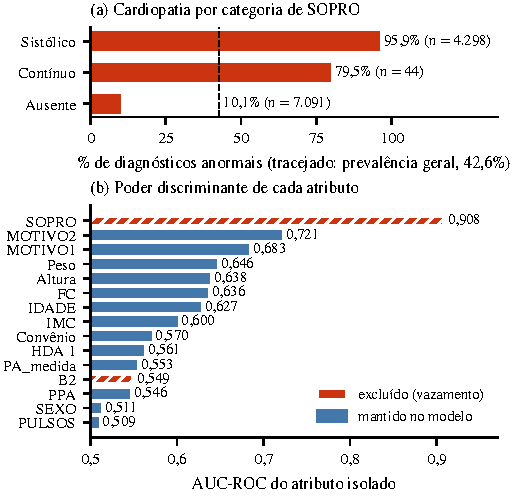
\includegraphics[width=\columnwidth]{fig1_eda.pdf}
\caption{(a) Prevalência de cardiopatia por categoria de SOPRO (categorias com $n\geq30$). (b) AUC-ROC de cada atributo isolado: nas categóricas, a taxa de anormais por categoria é aprendida no treino e aplicada ao teste das mesmas partições do experimento; nas numéricas, usa-se o próprio valor, nas linhas observadas. Em vermelho, os atributos excluídos por vazamento.}
\label{fig:eda}
\end{figure}

\textbf{De instância.} O dicionário chama o ID de ``identificador do paciente'', mas ele identifica o atendimento: \dado{retornos-pares} pares de IDs consecutivos têm a mesma data de nascimento e o mesmo sexo, contra \dado{retornos-acaso} esperados ao acaso. São retornos da mesma criança, e dividi-los entre treino e teste vazaria informação. Adotamos a chave de paciente DN\,+\,sexo, que forma \dado{grupos} grupos; há ainda \dado{mesmo-dia} grupos com mais de um registro no mesmo dia, \dado{mesmo-dia-divergente} deles com diagnósticos divergentes. A ordem dos IDs, por outro lado, não carrega o alvo (concordância entre vizinhos de \dado{ordem-id-concord}, contra \dado{ordem-id-acaso} ao acaso).

\textbf{De pré-processamento.} O arquivo limpo da A1 trazia valores imputados com medianas da base inteira. Esse arquivo foi abandonado: a imputação foi refeita dentro de cada partição de treino (Seção~\ref{sec:metodologia}).

Por fim, a prevalência de anormais cai de \dado{prev-ano-ini} em \dado{ano-ini} para \dado{prev-ano-fim} em \dado{ano-fim}. As datas ficaram fora do modelo, para que ele não aprenda a época em vez do paciente, mas essa deriva limita a generalização para períodos futuros.

\section{Metodologia}\label{sec:metodologia}

\begin{figure*}[t]
\centering
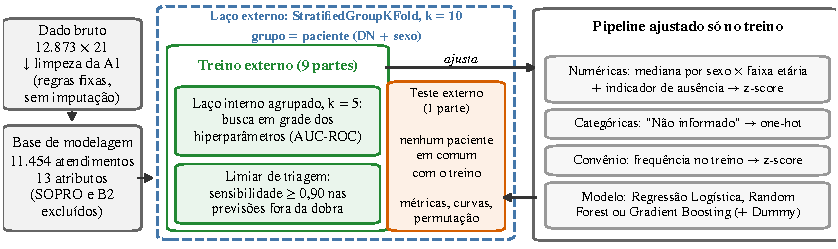
\includegraphics[width=\textwidth]{fig2_metodologia.pdf}
\caption{Pipeline e protocolo de validação. A limpeza usa apenas regras fixas e roda antes da partição; toda transformação com parâmetro é ajustada no treino de cada partição e só aplicada ao teste. Os atendimentos de uma mesma criança ficam inteiros de um dos lados.}
\label{fig:metodologia}
\end{figure*}

\subsection{Pré-processamento}

A limpeza segue a taxonomia da A1~\cite{tan2017}: sentinelas (zeros antropométricos, \texttt{\#VALUE!}, ``Indeterminado'') convertidos em ausência; valores fora de faixas clínicas tratados como ruído; datas em três formatos unificadas; IDADE e IMC recalculados; PPA reconstruída com as tabelas pediátricas de pressão arterial~\cite{nhbpep2004}; e remoção de registros sem alvo, duplicatas e contradições. Como são regras por registro ou critérios fixos, rodam antes da partição. A A2 acrescentou a padronização léxica do convênio, que reduziu as categorias de \dado{convenio-antes} para \dado{convenio-depois}.

As transformações com parâmetro formam um \textit{pipeline} ajustado só no treino de cada partição (Fig.~\ref{fig:metodologia}): (i) numéricas imputadas pela mediana do estrato sexo $\times$ faixa etária, com mediana global como reserva, mais um indicador de ausência por coluna --- a A1 mostrou que a falta de aferição é informativa --- e padronização \textit{z-score}, para que a penalidade L2 da logística não dependa da escala de cada medida (para as árvores, ela é inócua); (ii) categóricas, que são nominais e sem ordem, com a categoria explícita ``Não informado'' e codificação \textit{one-hot}; (iii) convênio codificado pela frequência no treino, evitando o \textit{target encoding}, que usaria o próprio alvo. Não houve reamostragem: o desbalanceamento é moderado, e o peso das classes entrou como hiperparâmetro.

\subsection{Validação e métricas}

A validação cruzada estratificada com $k=10$ é a referência da literatura~\cite{kohavi1995} e a diretriz prática da disciplina para $1.000 < N \leq 100.000$. Usamos \textbf{validação cruzada aninhada}: o laço externo (10 partições) estima o desempenho, e o interno (5 partições, dentro de cada treino externo) escolhe os hiperparâmetros por busca em grade com critério AUC-ROC. Os dois laços usam \texttt{StratifiedGroupKFold} com a chave de paciente, de modo que nenhum paciente, segundo essa chave, aparece em treino e teste. As partições são as mesmas para todos os modelos, e cada atendimento é avaliado uma única vez.

A classe positiva é \emph{Anormal}. A acurácia não serve de critério em classes desbalanceadas~\cite{faceli2021}; reportamos AUC-ROC (discriminação independente do limiar), AUC-PR (desempenho na classe positiva), acurácia balanceada, sensibilidade, especificidade, precisão e F1. Além do limiar 0,5, definimos um \textbf{limiar de triagem}: o maior limiar que atinge sensibilidade $\geq0{,}90$ nas previsões fora da dobra do próprio treino externo, aplicado depois ao teste --- o limiar nunca é escolhido olhando o teste.

\subsection{Algoritmos}

Comparamos: um piso de referência que prevê sempre a prevalência do treino; a \textbf{regressão logística} (LR) com regularização L2, \textit{baseline} simples e interpretável; e dois \textit{ensembles} de árvores, o \textbf{\textit{random forest}} (RF)~\cite{breiman2001} e o \textbf{\textit{gradient boosting}} (GB) baseado em histogramas~\cite{friedman2001,ke2017}, com parada antecipada. A Tabela~\ref{tab:hiper} traz o espaço de busca. A implementação usa scikit-learn~\cite{pedregosa2011}, pandas~\cite{mckinney2010}, NumPy~\cite{harris2020}, SciPy~\cite{virtanen2020} e Matplotlib~\cite{hunter2007}.

\begin{table}[t]
\centering
\caption{Espaço de busca e hiperparâmetros mais escolhidos nas 10 partições externas (LR: regressão logística; RF: \textit{random forest}; GB: \textit{gradient boosting})}
\label{tab:hiper}
\footnotesize
\begin{tabular}{@{}l>{\raggedright\arraybackslash}p{0.42\linewidth}>{\raggedright\arraybackslash}p{0.38\linewidth}@{}}
\toprule
Modelo & Espaço de busca & Valor mais escolhido (partições) \\
\midrule
LR & $C$ $\in$ \{0{,}01, 0{,}1, 1, 10\}; peso de classe $\in$ \{nenhum, balanceado\} & $C$ = 0{,}1 (8/10); peso de classe = balanceado (10/10) \\
\addlinespace
RF & prof. máx. $\in$ \{nenhum, 8, 16\}; mín. por folha $\in$ \{1, 5, 20\}; peso de classe $\in$ \{nenhum, balanceado\} & peso de classe = balanceado ou nenhum (5/10 cada); prof. máx. = 16 (9/10); mín. por folha = 5 (10/10) \\
\addlinespace
GB & taxa de aprend. $\in$ \{0{,}05, 0{,}1\}; folhas máx. $\in$ \{15, 31\}; reg. L2 $\in$ \{0, 1\}; peso de classe $\in$ \{nenhum, balanceado\} & peso de classe = balanceado (7/10); reg. L2 = 1 (8/10); taxa de aprend. = 0{,}05 (6/10); folhas máx. = 15 (10/10) \\
\bottomrule
\end{tabular}

\end{table}

\subsection{Comparação estatística}

Diferenças entre médias não bastam para declarar um modelo superior. Para um único conjunto de dados, aplicamos o \textbf{teste $t$ 5$\times$2cv} de Dietterich~\cite{dietterich1998}, que controla o erro Tipo I melhor que o teste $t$ sobre as partições de uma validação comum. Cada uma das 10 execuções repete o algoritmo inteiro, inclusive a busca interna, com metades formadas por grupos de paciente. O teste foi aplicado à AUC-ROC e à taxa de erro; os valores-$p$ dos três pares foram corrigidos por Holm~\cite{holm1979}, com $\alpha=0{,}05$.

\section{Resultados e discussão}

\begin{table*}[t]
\centering
\caption{Desempenho na validação cruzada aninhada agrupada (média $\pm$ desvio-padrão nas 10 partições externas). Em negrito, o melhor valor entre os três algoritmos (inclusive empates na precisão exibida).}
\label{tab:metricas}
\scriptsize
\setlength{\tabcolsep}{3.2pt}
\begin{tabular}{@{}lccccccccc@{}}
\toprule
 & \multicolumn{2}{c}{Independentes do limiar} & \multicolumn{4}{c}{Limiar 0{,}5} & \multicolumn{3}{c}{Limiar de triagem} \\
\cmidrule(lr){2-3}\cmidrule(lr){4-7}\cmidrule(l){8-10}
Modelo & AUC-ROC & AUC-PR & Acur. bal. & Sensib. & Especif. & F1 & Sensib. & Especif. & Precisão \\
\midrule
Classe majoritária & 0{,}500\,$\pm$\,0{,}000 & 0{,}426\,$\pm$\,0{,}000 & 0{,}500\,$\pm$\,0{,}000 & 0{,}000\,$\pm$\,0{,}000 & 1{,}000\,$\pm$\,0{,}000 & 0{,}000\,$\pm$\,0{,}000 & 1{,}000\,$\pm$\,0{,}000 & 0{,}000\,$\pm$\,0{,}000 & 0{,}426\,$\pm$\,0{,}000 \\
Regressão Logística & 0{,}770\,$\pm$\,0{,}014 & 0{,}715\,$\pm$\,0{,}021 & 0{,}708\,$\pm$\,0{,}010 & 0{,}623\,$\pm$\,0{,}019 & 0{,}794\,$\pm$\,0{,}019 & 0{,}656\,$\pm$\,0{,}013 & \textbf{0{,}899\,$\pm$\,0{,}012} & 0{,}341\,$\pm$\,0{,}007 & 0{,}503\,$\pm$\,0{,}004 \\
Random Forest & 0{,}785\,$\pm$\,0{,}015 & 0{,}734\,$\pm$\,0{,}026 & 0{,}715\,$\pm$\,0{,}009 & 0{,}610\,$\pm$\,0{,}037 & \textbf{0{,}819\,$\pm$\,0{,}028} & 0{,}658\,$\pm$\,0{,}017 & 0{,}898\,$\pm$\,0{,}014 & \textbf{0{,}400\,$\pm$\,0{,}012} & \textbf{0{,}527\,$\pm$\,0{,}006} \\
Gradient Boosting & \textbf{0{,}787\,$\pm$\,0{,}014} & \textbf{0{,}738\,$\pm$\,0{,}025} & \textbf{0{,}717\,$\pm$\,0{,}014} & \textbf{0{,}630\,$\pm$\,0{,}045} & 0{,}805\,$\pm$\,0{,}038 & \textbf{0{,}665\,$\pm$\,0{,}021} & \textbf{0{,}899\,$\pm$\,0{,}018} & 0{,}397\,$\pm$\,0{,}019 & 0{,}526\,$\pm$\,0{,}008 \\
\bottomrule
\end{tabular}

\end{table*}

\subsection{Desempenho comparado}

Os três algoritmos superam com folga o piso de referência (Tabela~\ref{tab:metricas}): a AUC-ROC sobe de \dado{dummy-aucroc} para valores entre \dado{logistica-aucroc} e \dado{gradientboosting-aucroc}, e a AUC-PR, de \dado{dummy-aucpr} para até \dado{gradientboosting-aucpr}. O \textit{gradient boosting} teve a maior AUC-ROC (\dado{gradientboosting-aucroc}\,$\pm$\,\dado{gradientboosting-aucroc-dp}), seguido de perto pelo \textit{random forest} (\dado{randomforest-aucroc}) e pela logística (\dado{logistica-aucroc}).

O teste 5$\times$2cv (Tabela~\ref{tab:testes}) indica que os dois \textit{ensembles} discriminam melhor que a logística ($p_{\mathrm{Holm}}$ de \dado{logistica-randomforest-aucroc-pholm} e \dado{logistica-gradientboosting-aucroc-pholm}); entre eles, não há diferença significativa ($p_{\mathrm{Holm}}=\dado{randomforest-gradientboosting-aucroc-pholm}$), o que não demonstra que sejam iguais. A vantagem, porém, é pequena --- de \dado{logistica-gradientboosting-aucroc-absdif} a \dado{logistica-randomforest-aucroc-absdif} de AUC --- e desaparece na taxa de erro no limiar 0,5, em que nenhum par difere ($p_{\mathrm{Holm}}\geq\dado{logistica-randomforest-erro-pholm}$). Os modelos não lineares ordenam melhor os pacientes, mas a convergência de três famílias de algoritmos para o mesmo patamar sugere que o limite está mais na informação disponível antes da ausculta do que no algoritmo. Por hiperparâmetro (Tabela~\ref{tab:hiper}), a escolha foi estável na logística ($C=\dado{hp-logistica-c}$ em \dado{hp-logistica-c-n} partições) e na estrutura das árvores (folha mínima de \dado{hp-randomforest-minsamplesleaf} no RF, \dado{hp-randomforest-minsamplesleaf-n}; \dado{hp-gradientboosting-maxleafnodes} folhas no GB, \dado{hp-gradientboosting-maxleafnodes-n}); já o peso de classe do RF se dividiu (balanceado em \dado{hp-randomforest-classweight-n}).

\begin{table}[t]
\centering
\caption{Teste $t$ 5$\times$2cv entre pares de algoritmos ($\overline{\Delta}$: média de A $-$ B nas 10 execuções; valores-$p$ corrigidos por Holm; siglas como na Tabela~\ref{tab:hiper})}
\label{tab:testes}
\footnotesize
\setlength{\tabcolsep}{3.5pt}
\begin{tabular}{@{}lccccc@{}}
\toprule
 & \multicolumn{3}{c}{AUC-ROC} & \multicolumn{2}{c}{Taxa de erro} \\
\cmidrule(lr){2-4}\cmidrule(l){5-6}
A $\times$ B & $\overline{\Delta}$ & $\tilde{t}$ & $p_{\mathrm{Holm}}$ & $\overline{\Delta}$ & $p_{\mathrm{Holm}}$ \\
\midrule
LR $\times$ RF & $-$0{,}012 & $-$4{,}57 & 0{,}018 & 0{,}008 & 0{,}536 \\
LR $\times$ GB & $-$0{,}011 & $-$3{,}44 & 0{,}037 & 0{,}006 & 0{,}666 \\
RF $\times$ GB & 0{,}001 & 0{,}42 & 0{,}695 & $-$0{,}002 & 0{,}597 \\
\bottomrule
\end{tabular}

\end{table}

\subsection{Limiar de decisão}

No limiar 0,5, o \textit{gradient boosting} tem sensibilidade de \dado{gradientboosting-sensibilidade} e especificidade de \dado{gradientboosting-especificidade}: perderia mais de um terço das cardiopatias, o que é inaceitável numa triagem. O limiar de triagem, escolhido no treino, ficou entre \dado{gradientboosting-limiarmin} e \dado{gradientboosting-limiarmax} e levou a sensibilidade média a \dado{trigradientboosting-sensibilidade} no teste (de \dado{trigradientboosting-sensibilidade-min} a \dado{trigradientboosting-sensibilidade-max} entre as partições), com especificidade de \dado{trigradientboosting-especificidade} e precisão de \dado{trigradientboosting-precisao} (Fig.~\ref{fig:curvas}). Em termos práticos, o modelo dispensaria \dado{tri-normais-dispensados-pct} das crianças normais da fila (\dado{matriztriagem-tn} de \dado{n-normal}), ao custo de deixar passar \dado{tri-cardiopatias-perdidas-pct} das cardiopatias (\dado{matriztriagem-fn} de \dado{n-anormal}). É um ganho de priorização, não um substituto do especialista.

\begin{figure}[t]
\centering
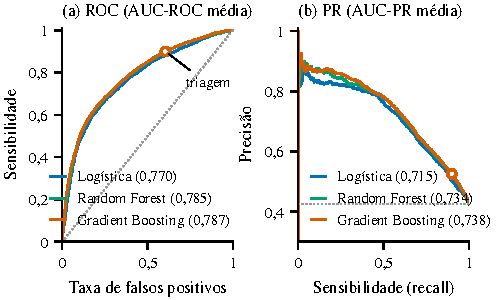
\includegraphics[width=\columnwidth]{fig3_curvas.pdf}
\caption{Curvas ROC e PR fora da dobra dos três algoritmos; o círculo marca o ponto de operação do \textit{gradient boosting} no limiar de triagem. Linhas pontilhadas: classificador sem informação.}
\label{fig:curvas}
\end{figure}

\subsection{Análise dos erros}

A Fig.~\ref{fig:erros}(a--b) mostra as matrizes de confusão agregadas do \textit{gradient boosting}. Os falsos negativos não se distribuem ao acaso: concentram-se onde o encaminhamento não traz sinal prévio. No limiar 0,5, o modelo perde \dado{perfilfn05-motivo1-5parecercardiologico} dos anormais encaminhados para parecer cardiológico (sobretudo avaliação pré-operatória) e \dado{perfilfn05-motivo1-2checkup} dos encaminhados para \textit{check-up}, contra \dado{perfilfn05-motivo1-1cardiopatiajaestabelecida} entre os que já chegam com cardiopatia estabelecida; no limiar de triagem, essas taxas caem para \dado{perfilfntriagem-motivo1-5parecercardiologico}, \dado{perfilfntriagem-motivo1-2checkup} e \dado{perfilfntriagem-motivo1-1cardiopatiajaestabelecida}. O erro também cresce com a idade: \dado{perfilfn05-faixaetaria-lactente} dos lactentes anormais são perdidos, contra \dado{perfilfn05-faixaetaria-adolescente} dos adolescentes. A ausculta segue indispensável: \dado{perfilfn05-pctfncomsopro} dos falsos negativos tinham sopro e seriam detectados por ela. Proporcionalmente, porém, o modelo erra mais nas cardiopatias sem sopro (perde \dado{perfilfn05-sopro-semsopro} delas, contra \dado{perfilfn05-sopro-comsopro} das com sopro; no limiar de triagem, \dado{perfilfntriagem-sopro-semsopro} contra \dado{perfilfntriagem-sopro-comsopro}), que dependem de outros achados do exame.

\begin{figure}[t]
\centering
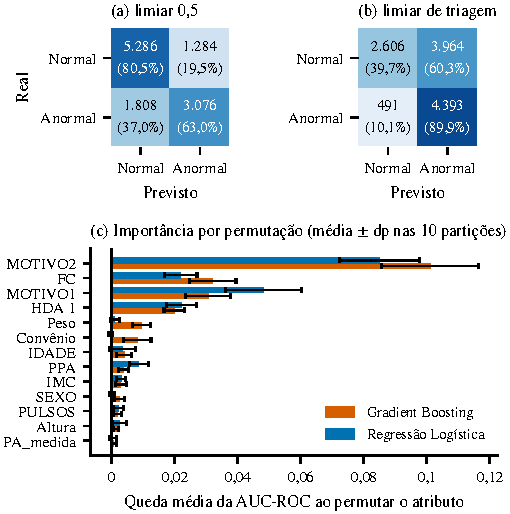
\includegraphics[width=\columnwidth]{fig4_erros.pdf}
\caption{Erros e importância. (a--b) Matrizes de confusão fora da dobra do \textit{gradient boosting}, com a taxa por linha. (c) Queda da AUC-ROC ao permutar cada atributo no teste de cada partição.}
\label{fig:erros}
\end{figure}

\subsection{Importância dos atributos}

A importância por permutação (Fig.~\ref{fig:erros}(c)) aponta o motivo do encaminhamento como o atributo dominante: permutar MOTIVO2 reduz a AUC do \textit{gradient boosting} em \dado{imp-gradientboosting-motivo2}, seguido de FC (\dado{imp-gradientboosting-fc}), MOTIVO1 (\dado{imp-gradientboosting-motivo1}) e HDA~1 (\dado{imp-gradientboosting-hda1}). Os coeficientes da logística dão o sentido do efeito. Como o modelo é regularizado e usa \textit{one-hot} completo, $e^{\beta}$ é um efeito relativo, sem categoria de referência única: o encaminhamento por sopro tem o maior efeito positivo ($e^{\beta}=\dado{or-catmotivo26sopro}$), seguido da cardiopatia já estabelecida (\dado{or-catmotivo11cardiopatiajaestabelecida}) e da congênita (\dado{or-catmotivo21cardiopatiacongenica}), enquanto \textit{check-up} (\dado{or-catmotivo12checkup}) e parecer cardiológico (\dado{or-catmotivo15parecercardiologico}) puxam o risco para baixo. O modelo aprende, essencialmente, a suspeita do médico que encaminhou, refinada pela frequência cardíaca e pelos sintomas --- clinicamente coerente e compatível com o patamar de desempenho observado. As medidas antropométricas, correlacionadas entre si, dividem a importância, que a permutação de uma de cada vez subestima.

\section{Conclusão}

O objetivo era estimar o risco de cardiopatia antes da ausculta. Sem vazamento, o \textit{gradient boosting} alcança AUC-ROC de \dado{gradientboosting-aucroc}, sem diferença significativa em relação ao \textit{random forest}; os \textit{ensembles} superam a regressão logística de forma estatisticamente significativa, mas por margem pequena, e, com sensibilidade de \dado{tri-sens-pct}, a especificidade fica em \dado{trigradientboosting-especificidade}. A conclusão prática é que esses dados permitem priorizar a fila do especialista, mas não substituir o exame que define o diagnóstico.

\textbf{Limitações.} Os dados vêm de um único hospital e quase todos de \dado{ano-ini} a \dado{ano-fim}, com prevalência em queda ao longo do período; a chave de paciente é aproximada, pois junta crianças nascidas no mesmo dia e não liga retornos sem data de nascimento ou sem sexo registrado; a população inclui \dado{sub-excluidos} encaminhamentos com cardiopatia já estabelecida, positivos fáceis para uma triagem --- sem eles, a AUC agregada cai de \dado{sub-auc-todos} para \dado{sub-auc} e a sensibilidade de triagem, de \dado{trigradientboosting-sensibilidade} para \dado{sub-sens}; a imputação reduz a variância das medidas; e MOTIVO2 depende da qualidade do encaminhamento, que pode variar entre serviços.

\textbf{Trabalhos futuros.} Validação temporal (treinar nos anos iniciais e testar nos finais), calibração das probabilidades, definição do limiar com os custos clínicos de cada erro e, sobretudo, a inclusão de fonocardiogramas obtidos por estetoscópio digital na triagem~\cite{oliveira2022}, que levaria ao modelo a informação do sopro sem depender do especialista.

\section*{Declaração de uso de IA generativa}

Ferramenta: Claude (Anthropic), via Claude Code. Onde e como: apoio na escrita do código Python do experimento, na geração das figuras e tabelas, na redação deste artigo e na produção dos slides. Para quê: acelerar a implementação e a produção do texto. As decisões metodológicas --- inclusive a exclusão de SOPRO e B2 --- e a interpretação dos resultados foram discutidas e aprovadas pelo grupo, e os resultados numéricos citados são gerados automaticamente a partir das saídas do código.

\bibliographystyle{IEEEtran}
\bibliography{referencias}

\end{document}
